\documentclass{article}

\usepackage[utf8]{inputenc}
\usepackage[T1]{fontenc}
\usepackage{hyperref}
\usepackage{url}
\usepackage{booktabs}
\usepackage{amsfonts}
\usepackage{nicefrac}
\usepackage{microtype}
\usepackage{nips_2017}
\usepackage{graphicx}
\usepackage{subcaption}
\usepackage{amsmath}
\usepackage{natbib}

\setcitestyle{numbers,open={[},close={]}}
\graphicspath{ {./images/} }

\title{Deep Multimodal Generative Models for Weakly-Supervised Learning}

\author{
    Mike Wu, Noah Goodman \\
    Department of Computer Science \\
    Stanford University \\
    \texttt{{wumike, ngoodman}@cs.stanford.edu} \\
}

\begin{document}

\maketitle

\begin{abstract}
TODO
\end{abstract}

\section{Introduction}
The problem of learning from multiple modalities is especially important since the majority of modern information is represented through multiple channels. For example, images in the web are often embedded around text. And while images can be described by pixels, we expect related modalities like text to also hold relevant features. People often interact with this multimodal information in a \textit{bi-directional} way. For example, one can imagine what a black cat looks like but also prescribe this description to a photo. Additionally, available multimodal information is often \textit{sparse}, in the sense there exist many large corpuses of images or text alone but few datasets exist (and are expensive to construct) that contain multiple modalities together. Ideally, we would like the generative models we build to extract a joint representation that captures high-level concepts across modalities in a way that is bi-directional and weakly-supervised. 

In this work, we propose a multimodal variational autoencoder (MMVAE). In our graphical model, we have two modalities $x_{1}$ and $x_{2}$ that are each conditioned on a latent variable $z$, which models the joint distribution, $p(x_{1}, x_{2})$. Such a modal is bi-directional since we can reconstruct both modalities from either $x_{1}$ or $x_{2}$. We will also show that we can train the MMVAE with sparse $(x_{1}, x_{2})$ pairs, and heavily utilize on a larger set of independent $(x_{1})$ and $(x_{2})$ examples. The most significant feature of MMVAEs is that it does not create a separate multimodal encoder $q(z | x_{1}, x_{2})$; instead it shares parameters with the encoders from each modality, $q(z | x_{1})$, $q(z | x_{2})$. This has the benefit of producing a simpler model while ensuring that high-dimensional missing modalities do not cause our generated samples to collapse.

\subsection{Related Work}
In deep learning, multimodal learning is often done using separate branches in the neural net for each modality, and a common top hidden layer. For instance, \citet{ngiam2011multimodal} trained deep autoencoders on audio and video input and found that the bimodal representations were better than any single equivalent. More recently, VAEs \cite{kingma2013auto, kingma2014semi} have been used to train models in high-dimensional multimodal settings. For example, conditional VAEs \cite{sohn2015learning} maximize a conditional log-likleihood by variational methods where often one modality is conditioned on another i.e. handwriting digits and labels, faces and attributes, or captioning. Notably, conditional VAEs (CVAE) are not bi-directional. 

\citet{pandey2017variational} proposed the conditional multimodal autoencoder (CMMA), which also maximizes a conditional log-likelihood. CMMA explicitly connects the conditional variable the latent variable, where CVAE does not. Moreover, it also constrains the latent representation to be close to the joint representation across modalities. However, CMMA is still not bi-directional.

Finally, \citet{suzuki2016joint} proposed a joint multimodal VAE (JMVAE). This is similar to our work in that it is bi-directional, handles missing modalities, and models the joint distribution. Our proposed model (MMVAE) and JMVAE share the same graphical notation, but differ in our approach. Crucially, JMVAE trains separate encoders for each modality and an additional one for the multimodal case. It then includes a KL divergence term \textit{per modality} in the loss. In constrast, MMVAE does not have an additional encoder for the multimodal case and does not have additional KL terms. It does so by sharing encoder parameters to learn the guide distributions: $q_{\phi_{x_{1}}}(z|x_{1})$, $q_{\phi_{x_{2}}}(z|x_{2})$, $q_{\phi}(z|x_{1}, x_{2})$

\section{Methods}
This section first briefly goes over VAEs, and product of Gaussians (PoG), then details a new multimodal VAE (MMVAE).

\subsection{Variational Autoencoders}
Variational autoencoders (VAE) model a generative process as $z \sim \mathcal{N}(0, I)$ and $x \sim p_{\theta}(x | z)$ where $x$ is an observed variable, $z$ is a latent variable, and $\theta$ are the model parameters. VAE wish to maximize the marginal distribution $p(x) = \int p_{\theta}(x | z)p(z)dx$, which is intractable. Instead, we maximize the lower bound of the marginal distribution:

\begin{equation}
    \textup{log } p(x) \geq -D_{KL}(q_{\phi}(z | x) || p(z)) + E_{q_{\phi}}[\textup{log } p_{\theta}(x | z)]
\end{equation}

where $q_{\phi}(z | x)$ is a \textit{guide distribution} that approximates the posterior $p(z | x)$; $\phi$ are the parameters of $q$. In the text, we call $p_{\theta}(x | z)$ a decoder and $q_{\theta}(z | x)$ an encoder. In practice, $q$ is set to the familiy of Gaussian distributions, where optimization amounts to learning $\phi=\{\mu, \sigma\}$. The standard reparametrization trick is employed to sample $z$.

\subsection{Product of Experts}

We wish to model the interaction between our modalities as a product of experts. Fortunately, because our guide distributions are Gaussian, MMVAEs take advantage of the fact the product of two Gaussian distributions is itself a Gaussian distribution \cite{cao2014generalized}. The mean and covariance of the resulting Gaussian distribution is:

\begin{equation}
    \mu = (\sum_{i} \mu_{i}\Sigma^{-1}_{i})(\sum_{i}\Sigma^{-1}_{i})^{-1}
\end{equation}
\begin{equation}
    \Sigma = (\sum_{i} \Sigma^{-1}_{i})^{-1}
\end{equation}

where $\mu_{i}$, $\Sigma_{i}$ is the mean and covariance of the $i$-th Gaussian expert.

\subsection{Multimodal Variational Autoencoders}
Given a dataset $(X_{1}, X_{2}) = \{ (x_{1,1}, x_{2,1}), ..., (x_{1,N}, x_{2,N}) \}$, where $x_{1}$ and $x_{2}$ are two modalities of possibly different dimensions. We assume that $x_{1}$ and $x_{2}$ are conditionally independent on the latent state $z$. Figure \ref{fig:diagram:graph} shows the graphical model of the generative process: $z \sim p(z)$ and $x_{1}, x_{2} \sim p(x_{1}, x_{2} | z)$.

We can estimate the lower bound of the log-likelihood $\textup{log }p(x_{1}, x_{2})$ as follows:

\begin{multline}
\textup{log }p(x_{1}, x_{2}) \geq -D_{KL}(q_{\phi}(z | x_{1}, x_{2}) || p(z)) \\ + E_{q_{\phi}(z | x_{1}, x_{2})}[\textup{log } p_{\theta_{x_{1}}}(x_{1} | z)] + E_{q_{\phi}(z | x_{1}, x_{2})}[\textup{log } p_{\theta_{x_{2}}}(x_{2} | z)]
\end{multline}

The equation above has two reconstruction terms, one for each modality. As with VAEs, we can parametrize the encoder and decoder as deep neural networks and use stochastic gradient descent to optimize the parameters, $\theta_{x_{1}}$, $\theta_{x_{2}}$, $\phi$. Because each modality learns a different feature representation, each modality has its own encoder and decoder.

In MMVAE, it is clear that we can compute the marginal and conditional distribution in both directions: given either $x_{1}$ or $x_{2}$ we can reconstruct both modalities. Additionally, we can easily extend MMVAE to handle more than two modalities, $p(x_{1}, x_{2}, ..., x_{n})$ using the same framework.

\begin{figure}[h!]
\centering
    \begin{subfigure}[b]{.24\linewidth}
        \centering
        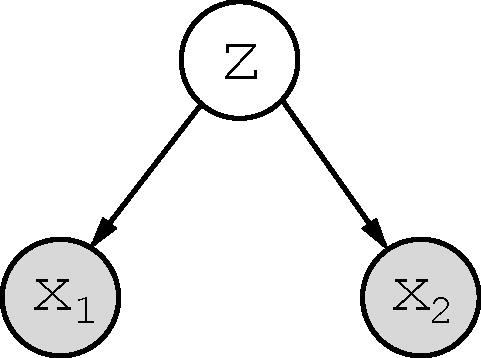
\includegraphics[width=.75\linewidth]{graph.pdf}
        \caption{}
        \label{fig:diagram:graph}
    \end{subfigure}\hspace{5mm}
    \begin{subfigure}[b]{.10\linewidth}
        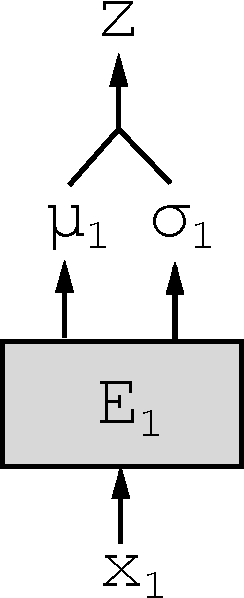
\includegraphics[width=.75\linewidth]{modelv2}
        \caption{}
        \label{fig:diagram:modelv2}
    \end{subfigure}\hspace{5mm}
    \begin{subfigure}[b]{.10\linewidth}
        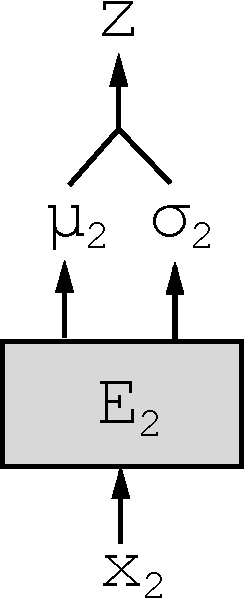
\includegraphics[width=.75\linewidth]{modelv1}
        \caption{}
        \label{fig:diagram:modelv1}
    \end{subfigure}\hspace{5mm}
    \begin{subfigure}[b]{.15\linewidth}
        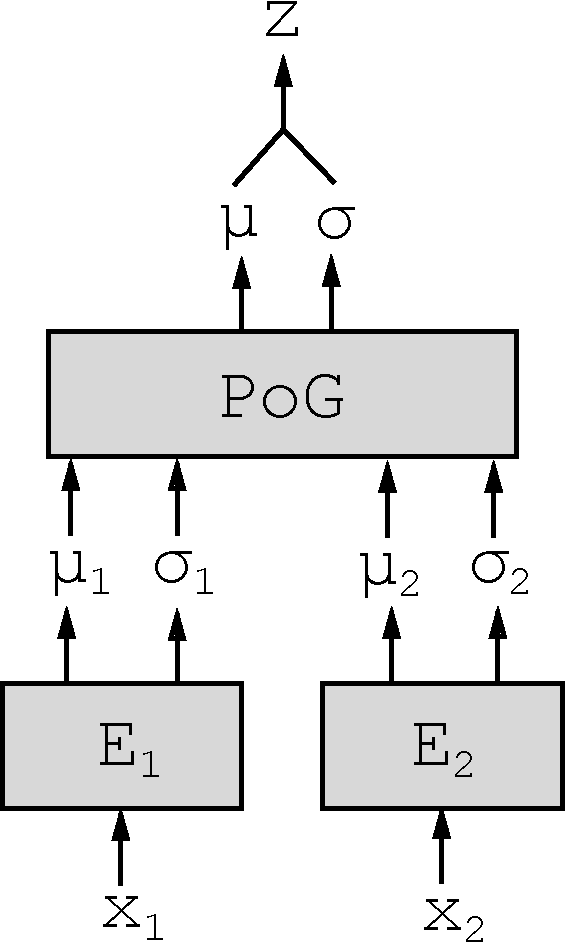
\includegraphics[width=.75\linewidth]{modelv3}
        \caption{}
        \label{fig:diagram:modelv3}
    \end{subfigure}
    \caption{(a) Graphical model of the MMVAE. Gray circles represent observed variables. The white circles represent latent variables. (b) MMVAE when modality 2 is missing. When only 1 modality is present, we ignore the PoG (product of Gaussians). (c) MMVAE when modality 1 is missing. (d) MMVAE when both modalities exist. $E_{1}$ and $E_{2}$ represent the two encoders: $q_{\phi_{x_{1}}}(z | x_{1})$ and $q_{\phi_{x_{2}}}(z | x_{2})$. Regardless if modalities are missing, we optimize the parameters of $E_{1}$ and $E_{2}$.}
    \label{fig:diagram}
\end{figure}

\subsection{Weakly-Supervised Training}
In most circumstances, paired modal data is both expensive and scarce while unimodal data, i.e. images or text is more easily available. The design of MMVAE allows for bootstrapping under sparse labels. During training, we consider input pairs of 3 types: the 1st modality alone,  the 2nd modality alone, or two separate modalities. Figure \ref{fig:diagram:modelv2}, \ref{fig:diagram:modelv1}, \ref{fig:diagram:modelv3} enumerate these three cases. In the case of a single modality, training is identical to VAE; the encoder $E_{i}(x_{i})$ returns $\mu_{i}$, $\sigma_{i}$, which is used to sample $z$ and decode. In the case of two modalities, each encoder returns $\mu_{i}$, $\sigma_{i}$, which we can combine via PoG to return the parameters of the joint Gaussian distribution. This is then used to sample $z$ and decode as in the traditional VAE. Crucially, we do not need additional loss terms or separate networks to handle unimodal and multimodal cases; the only change required is an additional PoG operation. In practice, we find that we only need a limited amount of paired multimodal examples in order to learn the cross-modal relations. 

\bibliographystyle{abbrvnat}
{\small
\linespread{1}
\bibliography{draft}
}

\end{document}